\begin{tikzpicture}
    \begin{axis}[
    ybar,
    width=\linewidth, height=5cm,
    ylabel={$a(h, b, r)$}, ylabel near ticks, ymin=0, ymax=1.3,
    xtick={1, 2, 3}, xticklabels={$\ang{0}$, $\ang{0.0001}$, $\ang{0.01}$},
    xlabel={$\rho$ (degrees)}, xmin=0.5, xmax=3.5, xtick pos=left,
    nodes near coords, every node near coord/.append style={rotate=90, anchor=west},
    legend style={at={(0.5,-0.35)}, anchor=north,legend columns=-1},
    bar width=7
    ]
        \addplot coordinates {(1, 0.977) (2, 0.973) (3, 0.004)};
        \addplot coordinates {(1, 1.0) (2, 1.0) (3, 0.706)};
        \addplot coordinates {(1, 1.0) (2, 0.814) (3, 0.025)};
        \addplot coordinates {(1, 1.0) (2, 0.862) (3, 0.025)};
        \addplot coordinates {(1, 0.999) (2, 0.999) (3, 0)};
        \addplot coordinates {(1, 1.0) (2, 0.003) (3, 0)};
        \legend{ANG, DOT, SPH, PLN, PYR, COM}
    \end{axis}
\end{tikzpicture}